% Auriga theme
% find the most up-to-date version here: https://github.com/anishathalye/auriga

\documentclass[14pt,aspectratio=169]{beamer}
\usepackage{pgfpages}
\usepackage{fancyvrb}
\usepackage{tikz}
\usepackage{pgfplots}
\usepackage{booktabs}

% Use natbib with author-year citation style
%\usepackage[authoryear]{natbib}

% Add the bibliography style compatible with author-year
%\bibliographystyle{plainnat}

\setbeamertemplate{bibliography item}[text]

\renewcommand{\footnote}[1]{
    \begin{tikzpicture}[remember picture,overlay]
        \node[anchor=north east, xshift=-0.2cm, yshift=-0.2cm] at (current page.north east) {\footnotesize #1};
    \end{tikzpicture}
}
\usetheme{auriga}
\usecolortheme{auriga}
\setbeamercolor{math text}{fg=blue}

\newcommand\blfootnote[1]{%
\begingroup
\renewcommand\thefootnote{}\footnote{#1}%
\addtocounter{footnote}{-1}%
\endgroup
}

%\setbeamertemplate{footline}[]
%\renewcommand\footnotemark{}


% define some colors for a consistent theme across slides
\definecolor{red}{RGB}{181, 23, 0}
\definecolor{blue}{RGB}{0, 118, 186}
\definecolor{gray}{RGB}{146, 146, 146}
\title{Speculations \\ on \\ Test-Time Scaling}
\author{Sasha Rush \  Daniel Ritter}

\institute[shortinst]{Cornell}
% \institute[shortinst]{\inst{*} Preprint}


\begin{document}

\frame{\titlepage}

\begin{frame}{Outline}
	\tableofcontents[sections]
\end{frame}

\section{Introduction}

\begin{frame}[t]{}
	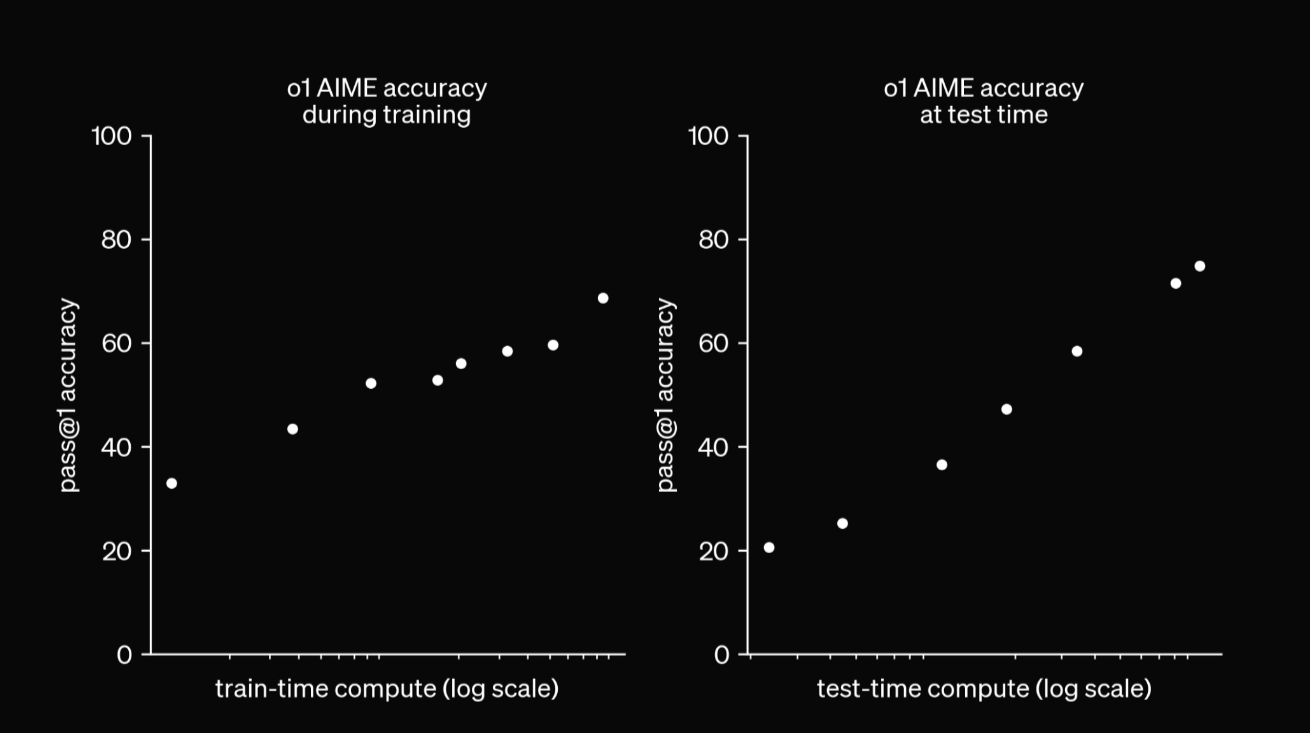
\includegraphics[width=\linewidth]{images/compute.png}
\end{frame}

\begin{frame}{Context}
	\begin{itemize}
		\item LLM (2018-2024) driven by training scaling
		\item Speculation: Benefit of static data running out
	\end{itemize}
	\blfootnote{}
\end{frame}

\begin{frame}{Implication}
	\begin{itemize}
		\item Breakthrough in large-scale RL Training
		\item
	\end{itemize}
	\blfootnote{}
\end{frame}

\begin{frame}{What have we seen?}
	\begin{itemize}
		\item Public demo model
		\item Strong result in constrained domains.
	\end{itemize}
	\blfootnote{}
\end{frame}

\begin{frame}{This Talk}
	\begin{itemize}
		\item Survey of the public literature
		\item Synthesis of discussions with expert
		\item Gossip and hearsay
	\end{itemize}
	\blfootnote{}
\end{frame}

\begin{frame}{Thanks}
	Lewis Tunstall, Edward Beeching, Aviral Kumar, Charlie Snell,
	Michael Hassid, Yoav Artzi, Risab Agarwal, Kanishk Gandhi,
	Wenting Zhao, Yuntian Deng, Nathan Lambert
\end{frame}

\section{The Clues}

\begin{frame}{What we know}
	Our large-scale \textbf{reinforcement learning algorithm} teaches the model
	how to think productively using its \textbf{chain of thought} in a highly
	\textbf{data-efficient} training process.
\end{frame}

\begin{frame}{What we know}
	\begin{itemize}
		\item RL - Signal from verifiable problems
		\item CoT - ``Thinking'' occurs in token stream
		\item Data Efficient - Fixed set of good problems
	\end{itemize}
\end{frame}

\begin{frame}{From Gossip}
	\begin{itemize}
		\item Single final model
		\item Not learned from expert examples
		\item
	\end{itemize}
\end{frame}

\begin{frame}{Chain of Thought}
	o1 learns to hone its chain of thought and refine the strategies it uses.
	It learns to recognize and \textbf{correct its mistakes}.
	It learns to \textbf{break down tricky steps} into simpler ones.
	It learns to try a \textbf{different approach} when the current one isn’t working.
\end{frame}

\begin{frame}{Review: Chain of Thought}
	\begin{itemize}
		\item
	\end{itemize}
	\blfootnote{}
\end{frame}

\begin{frame}{Planning}
\end{frame}

\begin{frame}{Backtracking}
\end{frame}

\begin{frame}{Strategies}
\end{frame}


\begin{frame}{Summary}
	\begin{itemize}
		\item Solves problems by very long CoT
		\item CoT includes ``thinking'' (search / planning)
		\item Core novelty: Inducing this behavior
	\end{itemize}
\end{frame}

\section{Notation}

\begin{frame}{Notation - Test-Time (No learning yet!)}
	\begin{itemize}
		\item $x$ - a conditional question
		\item $z \in {\mathcal{S}^T}$ - the chain of thought
		\item $y \in {\mathcal Y}$ - the response
		\item $p(y | x) = E_{z \sim p(x|z)} p(y|x,z)  $ - model
	\end{itemize}
\end{frame}

\begin{frame}{Warm-up: Ancestral Sampling}
	\begin{itemize}
		\item \tilde{z} \cite p(z | x)
		\item \tilde{y} \cite p(y | x, \tilde{z})
	\end{itemize}

	$|\tilde{z}|$ amount of test-time compute
\end{frame}

\begin{frame}{Warm-up: Monte-Carlo (Self-Consistency)}
	\begin{itemize}
		\item \tilde{z} \cite p(z | x)
		\item \tilde{y} \cite p(y | x, \tilde{z})
	\end{itemize}
	Pick $\argmax_{} y = \tilde{y}$
\end{frame}

\begin{frame}{Warm-up: Beam Search}
	\begin{itemize}
		\begin{itemize}
			\item \tilde{z} \cite p(z | x)
		\end{itemize}
		\item \tilde{y} \cite p(y | x, \tilde{z})
	\end{itemize}
\end{frame}

\begin{frame}{Notation - Verifier}
	\begin{itemize}
		\item $\text{Ver} : \mathcal{Y} \rightarrow \{0, 1}$
		\item $z \in {\mathcal{S}^T}$ - the chain of thought
		\item $y$ - the response
		\item $p(y | x) = E_{z \sim p(x|z)} p(y|x,z)  $ - model
	\end{itemize}
\end{frame}


\begin{frame}{Warm up: Rejection Sampling}
	\begin{itemize}
		\item \tilde{z} \cite p(z | x)
		\item \tilde{y} \cite p(y | x, \tilde{z})
	\end{itemize}
\end{frame}


\begin{frame}{Warm up: Monte-Carlo Roll-Outs}
	Start at $z$
	\begin{itemize}
		\item \tilde{z} \cite p(z | x, z)
		\item \tilde{y} \cite p(y | x, \tilde{z})
	\end{itemize}
\end{frame}


\begin{frame}{Goal: Learning}
	\begin{itemize}
		\item $\max_{theta} \sum \log p(y | x; \theta)$
		\item Intractable expectation over latent CoT
	\end{itemize}
\end{frame}




\section{The Suspects}

\begin{frame}{Outline}
	\tableofcontents[sections]
\end{frame}

\begin{frame}{The Suspects}
	\begin{itemize}
		\item Guess + Check
		\item Guided Search
		\item AlphaZero
		\item Learn to Search
		\item Wildcard
	\end{itemize}

\end{frame}

\begin{frame}{A Note About Names}
	\begin{itemize}
		\item Many different communities
		\item Names conflict and overlap with past methods
		\item This talk: First explain, then discuss names
	\end{itemize}
\end{frame}


\begin{frame}{Offline / Online?}
	\begin{itemize}
		\item Each approach has two variants
		\item I will describe offline/batch variant
		\item Companies have complex internal RL optimizers to make online variant works
	\end{itemize}
\end{frame}


\subsection{Guess and Check}

\begin{frame}{Informal: Guess + Check}
	\begin{itemize}
		\item Sample N CoTs
		\item Check if successful
		\item Train on good ones
	\end{itemize}
\end{frame}

\begin{frame}{Formalization: EM}
	\begin{itemize}
		\item $$\max_{theta} \sum \log p(y | x; \theta) = \sum \log E_{z} p(y, z | x)$$
		\item E-Step: Compute $p(z | y, x) \propto (Ver(y)) p(z | x) $
		\item M-Step: Fit $p(y, z | x)$
	\end{itemize}
	Hard EM
\end{frame}


\begin{frame}{Offline}
	\begin{itemize}
		\item Batch servers to sample
		\item Check if successful
		\item Train on good ones
	\end{itemize}
\end{frame}


\begin{frame}{Online}
	\begin{itemize}
		\item Sample N CoTs
		\item Check if successful
		\item Train on good ones
	\end{itemize}
\end{frame}


\begin{frame}{Terminology}
	\begin{itemize}
		\item STaR
		\item ReST
		\item ReST-EM
		\item Filtered Rejection Sampling
		\item Best-of-N
	\end{itemize}
\end{frame}


\begin{frame}{Why might this be right?}
	\begin{itemize}
		\item Extremely simple and scalable
		\item Good baseline in past work
	\end{itemize}
\end{frame}

\begin{frame}{Why might this be wrong?}
	\begin{itemize}
		\item No evidence this learns to correct, plan
		\item Well-explored in literature with marginal gains
	\end{itemize}
\end{frame}

\begin{frame}{Alternative}
	\begin{itemize}
		\item Can we improve upon the process of finding adequate CoTs?
	\end{itemize}
\end{frame}


\subsection{Guided Search}

\begin{frame}{Informal: Guided Search}
	\begin{itemize}
		\item Sample several next steps for CoT
		\item Check with a guide model for which to pursue
		\item Continue to the end
		\item Train on good ones
	\end{itemize}
\end{frame}


\begin{frame}{Warm-up: Beam Search with Roll-Outs}
	\begin{itemize}
		\begin{itemize}
			\item \tilde{z} \cite p(z | x)
		\end{itemize}
		\item \tilde{y} \cite p(y | x, \tilde{z})
	\end{itemize}
\end{frame}

\begin{frame}{Where does the guide come from?}


\end{frame}

\begin{frame}{PRM/RollOuts}
	\begin{itemize}
		\item Point 1
		\item Point 2
		\item Point 3
	\end{itemize}
	\blfootnote{\cite{Uesato2022-aw}}
\end{frame}


\begin{frame}{Why might this be right?}
	\begin{itemize}
		\item Major demonstrated RL result
		\item
	\end{itemize}
\end{frame}

\begin{frame}{Why might this be wrong?}
	\begin{itemize}
		\item Does not inject into CoT
		\item Relatively complex to scale
	\end{itemize}
\end{frame}


\begin{frame}{Alternative}
	\begin{itemize}
		\item Can we improve on the search?
	\end{itemize}
\end{frame}

\subsection{AlphaZero}

\begin{frame}{Reminder: AlphaZero}

\end{frame}

\begin{frame}{Informal: AlphaZero}
	\begin{itemize}
		\item Search for best solution with model
		\item Collect the best CoT
		\item Train on good ones
	\end{itemize}
\end{frame}

\begin{frame}

\end{frame}

\begin{frame}{Formalized: Expert Iteration}
	\begin{itemize}
		\item
	\end{itemize}
	\blfootnote{\cite{Anthony2017-dm}}}
\end{frame}


\begin{frame}{Why might this be right?}
	\begin{itemize}
		\item Major demonstrated RL result
		\item
	\end{itemize}
\end{frame}

\begin{frame}{Why might this be wrong?}
	\begin{itemize}
		\item Does not inject into CoT
		\item Relatively complex to scale
	\end{itemize}
\end{frame}


\begin{frame}{Alternative}
	\begin{itemize}
		\item Can we get the CoT to search?
	\end{itemize}
\end{frame}


\section{Learning to Correct}

\begin{frame}{Challenge}

\end{frame}

\begin{frame}{Informal: Learning to Correct}
	\begin{itemize}
		\item Find optimal paths
		\item Adjust to add mistakes
		\item
	\end{itemize}
\end{frame}


\begin{frame}{Formalized: Stream of Search}
	\begin{itemize}
		\item
		\item
		\item
	\end{itemize}
	\blfootnote{\cite{Gandhi2024-vs}}
\end{frame}

\begin{frame}{Formalized: Advantage}
	\begin{itemize}
		\item
		\item
		\item
	\end{itemize}
\end{frame}

\begin{frame}{Why might this be right?}
	\begin{itemize}
		\item
		\item
	\end{itemize}
\end{frame}

\begin{frame}{Why might this be wrong?}
	\begin{itemize}
		\item
		\item
	\end{itemize}
\end{frame}

\section{Wild}

\begin{frame}{No Supervision}
	\begin{itemize}
		\item
	\end{itemize}
	\blfootnote{\cite{Brown2024-bs}}
\end{frame}


\begin{frame}{MuZero}
	\begin{itemize}
		\item
	\end{itemize}
	\blfootnote{\cite{Brown2024-bs}}
\end{frame}

\section{Implications}

\begin{frame}{}
	\begin{itemize}
		\item
	\end{itemize}
	\blfootnote{\cite{Brown2024-bs}}
\end{frame}

\begin{frame}[allowframebreaks]{Reference}
	\bibliographystyle{apalike}
	\bibliography{../o1.bib}
\end{frame}

\end{document}
